\documentclass[a4paper, 10pt]{article}
\linespread{1.0} %interlinea
\usepackage{geometry} %margini
\usepackage[]{tabto}
\geometry{a4paper, top=3cm, bottom=3cm, left=3cm, right=3cm, bindingoffset=5mm}
\usepackage{graphicx}
\usepackage{adjustbox}
\graphicspath{Documentazione/Immagini/}
\usepackage{multicol} %più colonne
\usepackage{ragged2e} %allineamento testo
\usepackage{float}
\usepackage{inconsolata}
\usepackage[]{fancyhdr}
\usepackage[utf8]{inputenc}
\usepackage{array}
\usepackage{tabularx}
\usepackage{enumitem}
\usepackage{multirow}
\usepackage{longtable}
\usepackage{tcolorbox}
\usepackage{xcolor, listings}
\usepackage[T1]{fontenc}
\usepackage{lmodern}
\tcbuselibrary{skins}
\renewcommand{\familydefault}{\sfdefault}
\geometry{margin=2.3cm}
\renewcommand{\arraystretch}{1.2} % Aumenta altezza delle righe
\setlist[itemize]{left=0pt, label=\textbullet, itemsep=1pt, topsep=1pt}
\definecolor{linecolor}{RGB}{200, 200, 200}

\newtcolorbox{graybox}{
	colback=gray!15,
	colframe=gray!15,
	boxrule=0pt,
	left=1em,
	top=4pt,          % Spazio interno superiore
	bottom=4pt,       % Spazio interno inferiore
	before skip=4pt,  % Spazio prima del box
	after skip=6pt,   % Rimuove spazio aggiuntivo automatico
	enhanced,
	sharp corners
}
\usepackage{listings}
\usepackage{xcolor}

% Colori coerenti con l'immagine
\definecolor{sqlgreen}{rgb}{0,0.5,0}
\definecolor{sqlblack}{rgb}{0,0,0}
\definecolor{sqlblue}{rgb}{0,0,0.7}
\definecolor{sqlpurple}{rgb}{0.58,0,0.82}
\definecolor{sqlgray}{rgb}{0.5,0.5,0.5}
\definecolor{sqlbg}{rgb}{0.98,0.98,0.98}

\lstdefinestyle{sqlstyle}{
	language=SQL,
	backgroundcolor=\color{sqlbg},
	basicstyle=\footnotesize\ttfamily,
	commentstyle=\color{sqlgreen}\itshape,
	keywordstyle=\color{sqlblue}\bfseries,
	stringstyle=\color{sqlpurple},
	showstringspaces=false,
	numbers=left,
	numberstyle=\tiny\color{sqlblack},
	numbersep=2pt,
	breaklines=true,
	tabsize=2,
	frame=single,
	rulecolor=\color{black},
	framerule=0.5pt,
	xleftmargin=15pt,
	framexleftmargin=10pt,
	aboveskip=10pt,
	belowskip=10pt,
	morekeywords={
		CREATE, TABLE, PRIMARY, KEY, FOREIGN, REFERENCES,
		CONSTRAINT, CHECK, VARCHAR, INTEGER, DATE, NOT, NULL,
		AND, OR, BEGIN, END, IF, THEN, ELSE, RETURN, DEFAULT
	}
}

% \begin{lstlisting}[style=sqlstyle]
	%   Il tuo codice SQL qui
	% \end{lstlisting}

\pagestyle{fancy}
\fancyhead{}
\cfoot{\thepage}
\lfoot{Gioele Manzoni}
\rfoot{Luca Lucci}
\author{Gioele Manzoni}
\title{Documentazione per Progettazione Base di Dati}
\begin{document}
	\begin{center}
		\begin{figure}[hb]
			
\includegraphics[width=1\textwidth]{../Immagini/coverpic.png}
		\end{figure}
		{\LARGE DOCUMENTAZIONE PER PROGETTAZIONE \\BASE DI DATI \par}
		{\Large{Progetto in Carico: Hackathon \par}}
		\vfill
		{\large{\textbf{\textsc{CdL Triennale in Informatica}}}}\\
		{\large{\textsc{Corso di Basi di Dati I}}}\\
		{\large{\textsc{GIOELE MANZONI}}}\\
		{\large{\textsc{N86004562}}}\\
		{\large{\textsc{LUCA LUCCI}}}\\
		{\large{\textsc{N86005180}}}\\
		{\large{\textsc{\today}}}\\
		\Large{\textsc{Anno Accademico: 2024/2025}}
	\end{center}
	\newpage
	\tableofcontents
	\newpage
	\section{Introduzione}
	Questa documentazione descriverà il processo di progettazione e sviluppo di un Database relazionale che gestirà il flusso di dati di un applicativo dedicato all'organizzazione di Hackathon. Questo è un progetto a cura degli studenti Gioele Manzoni e Luca Lucci del CdL di Informatica presso l'Università degli Studi di Napoli "Federico II".
	\subsection{Traccia del Progetto}
	Un hackathon, ovvero una "maratona di hacking", è un evento durante il quale team di partecipanti si sfidano per progettare e implementare nuove soluzioni basate su una certa tecnologia o mirate a un certo ambito applicativo. 
	Ogni hackathon ha un titolo identificativo, si svolge in una certa sede e in un certo intervallo di tempo (solitamente 2 giorni) e ha un organizzatore specifico (registrato alla piattaforma). L'organizzatore seleziona un gruppo di giudici (selezionati tra gli utenti della piattaforma, invitandoli). Infine, l'organizzatore apre le registrazioni, che si chiuderanno 2 giorni prima dell'evento. Ogni evento avrà un numero massimo di iscritti e una dimensione massima del team.
	Durante il periodo di registrazione, gli utenti possono registrarsi per l'Hackathon di loro scelta (eventualmente registrandosi sulla piattaforma se non lo hanno già fatto). Una volta iscritti, gli utenti possono formare team. I team diventano definitivi quando si chiudono le iscrizioni. All'inizio dell'hackathon, i giudici pubblicano una descrizione del problema da affrontare. 
	Durante l'hackathon, i team lavorano separatamente per risolvere il problema e devono caricare periodicamente gli aggiornamenti sui "progressi" sulla piattaforma come documento, che può essere esaminato e commentato dai giudici. Alla fine dell'hackathon, ogni giudice assegna un voto (da 0 a 10) a ciascun team e la piattaforma, dopo aver acquisito tutti i voti, pubblica le classifiche dei team.
	\subsection*{Caratteristiche dell'Hackathon}
	Ogni Hackathon ha le seguenti caratteristiche:
	\begin{itemize}
		\item Un \textbf{titolo identificativo};
		\item Una \textbf{sede} in cui si svolge;
		\item Un \textbf{intervallo di tempo}, solitamente di due giorni;
		\item Un \textbf{organizzatore specifico}, registrato sulla piattaforma.
	\end{itemize}
	\subsection*{Giudici e Registrazioni}
	\begin{itemize}
		\item L'organizzatore seleziona un gruppo di \textbf{giudici}, invitandoli tra gli utenti registrati sulla piattaforma.
		\item L'organizzatore apre le \textbf{registrazioni}, che si chiudono due giorni prima dell'inizio dell'evento.
		\item Ogni evento prevede un \textbf{numero massimo di iscritti} e una \textbf{dimensione massima del team}.
		\item Durante il periodo di registrazione, gli utenti possono registrarsi all'Hackathon di loro scelta, previa registrazione sulla piattaforma se non ancora effettuata.
	\end{itemize}
	\subsection*{Formazione dei Team}
	\begin{itemize}
		\item Una volta iscritti, gli utenti possono \textbf{formare team}.
		\item I team diventano \textbf{definitivi alla chiusura delle iscrizioni}.
	\end{itemize}
	\subsection*{Svolgimento dell'Hackathon}
	\begin{itemize}
		\item All'inizio dell'evento, i giudici \textbf{pubblicano una descrizione del problema} da affrontare.
		\item Durante l’Hackathon, i team lavorano separatamente per risolvere il problema.
		\item I team devono \textbf{caricare periodicamente aggiornamenti sui progressi} tramite documenti sulla piattaforma.
		\item I documenti possono essere \textbf{esaminati e commentati dai giudici}.
	\end{itemize}
	\subsection*{Valutazione e Classifica}
	\begin{itemize}
		\item Alla fine dell'Hackathon, ogni giudice assegna un \textbf{voto da 0 a 10} a ciascun team.
		\item La piattaforma, dopo aver acquisito tutti i voti, \textbf{pubblica le classifiche dei team}.
	\end{itemize}
	\section{Progettazione Concettuale}
	\subsection{Analisi delle Entità e degli Attributi}
	Seguendo la traccia, nella fase di progettazione concettuale sono state trovate le suddette entità:
	\subsubsection{Hackathon}
	Entità dedicata a tutte le maratone di Hacking organizzate.
	\begin{itemize}
		\item \textbf{Hackathon} ($\underline{Titolo\_identificativo}$, Descrizione\_problema, Sede, Classifica,\\ DataInizio\_registrazioni, DataFine\_registrazioni, DataInizio\_Evento, DataFine\_Evento, \\Num\_iscrittiCorrente, MaxNum\_membriTeam, MaxNum\_iscritti)
	\end{itemize}
	\subsubsection{Utente}
	Generalizzazione dedicata a tutti i tipi di utenti che è possibile avere all'interno della piattaforma.
	La generalizzazione è considerata come \textbf{DISGIUNTA PARZIALE}, poiché è possibile avere utenti della piattaforma che non sono né organizzatori né giudici.
	\begin{itemize}
		\item \textbf{Utente} ($\underline{Login}$, Password)
	\end{itemize}
	\subsubsection{Organizzatore}
	Specializzazione dell'entità \textbf{Utente}, rappresentante gli organizzatori di maratone di Hacking.
	Non possiede alcun attributo specifico a sé stesso, la sua specializzazione definisce soltanto gli utenti con le giuste credenziali per poter gestire la piattaforma.
	\subsubsection{Giudice}
	Specializzazione dell'entità \textbf{Utente}, rappresentante i giudici che daranno le loro valutazioni ai documenti e supervisioneranno le Hackathon.
	\subsubsection{Team}
	Entità che definisce una squadra organizzata da un Utente e composta da N Utenti.
	\begin{itemize}
		\item \textbf{Conferenza} ($\underline{NomeTeam}$, VotoFinale)
	\end{itemize}
	\subsubsection{Documento}
	Entità debole che definisce un documento scritto da un team.
	\begin{itemize}
		\item \textbf{Documento} ($\underline{NomeTeam}$, Testo)
	\end{itemize}
	\subsection{Analisi delle Relazioni}
	Qui verranno descritte tutte le relazioni e le specializzazioni presenti all'interno della struttura concettuale non ancora ristrutturata.
	\begin{itemize}
		\item \textit{Organizzazione} (\textbf{Hackathon} - \textbf{Organizzatore}: 1 - N):\\Un Hackathon può essere organizzata da un solo organizzatore. Un organizzatore può organizzare più Hackathon.
		\item \textit{Partecipazione} (\textbf{Team} - \textbf{Hackathon}: 1 - 2..N):\\Un Team può partecipare ad una sola Hackathon. Un Hackathon, per essere valida, deve avere un minimo di 2 Team fino ad un massimo di N.
		\item \textit{Supervisione} (\textbf{Giudice} - \textbf{Hackathon}: 1..N - N):\\Un Giudice può supervisionare N Hackathon. Un Hackathon deve essere monitorata da almeno un giudice.
		\item \textit{Appartenenza} (\textbf{Utente} - \textbf{Team}: 0..N - 1..N):\\Un Utente può partecipare ad uno o più team, o può non parteciparci affatto. Un Team deve essere composto da un minimo di un Utente fino ad un massimo di N (il limite di utenti appartenenti ad un Team è deciso dall'Hackathon alla quale si partecipa).
		\item \textit{Invito} (\textbf{Giudice} - \textbf{Hackathon}: 1..N - 1..N):\\Un giudice deve invitare un minimo di un utente fino ad un massimo di N utenti per essere giudici. Un giudice, per ricevere un invito, deve riceverlo da almeno un organizzatore.
		\item \textit{Voto} (\textbf{Giudice} - \textbf{Team}: 1..N - 1..N):\\Un Giudice può esprimere una votazione ad un minimo di un Team. Un team può ricevere voti da almeno un giudice.
		\item \textit{Valutazione} (\textbf{Giudice} - \textbf{Documento}: 1..N - 1..N):\\Un Giudice deve esprimere una valutazione per almeno un documento. Un documento deve ottenere una valutazione da almeno un giudice.
		\item \textit{Pubblicazione} (\textbf{Documento} - \textbf{Team}: 1 - N):\\Relazione identificante per l'entità debole Documento, in quanto generato direttamente da un Team e non può esistere senza un associazione ad un Team.
	\end{itemize}
	\begin{figure}[H]
		\centering
		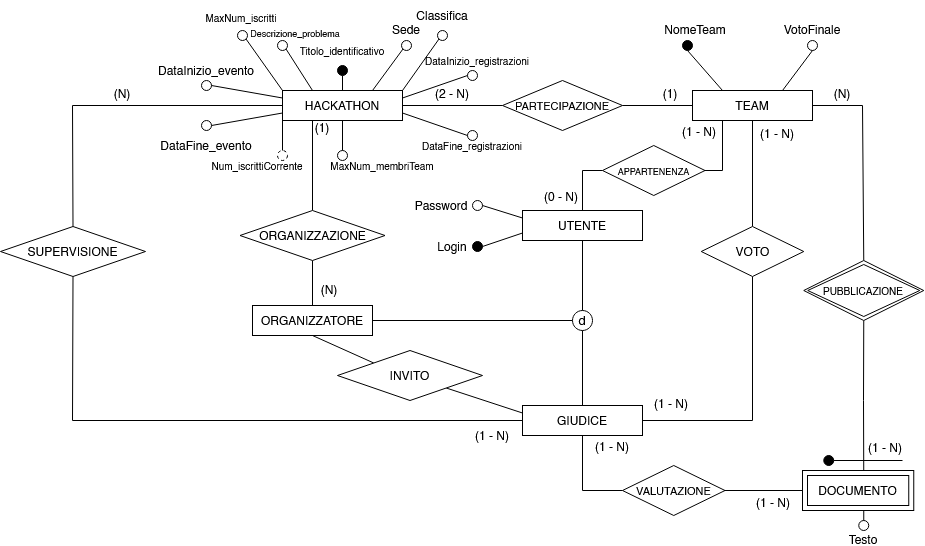
\includegraphics[width=1\textwidth]{../Immagini/EERDiagram_Hackathon}
		\caption[Grafico UML]{Grafico EER Concettuale}
	\end{figure}
	\newpage
	\section{Ristrutturazione Modello Concettuale}
	\subsection{Ristrutturazione del Modello Concettuale}
	Dopo aver analizzato i requisiti, le entità e le relazioni ed aver prodotto uno schema concettuale passeremo alla sua Ristrutturazione, seguendo i passaggi necessari elencati nelle prossime sottosezioni, ordinate in:
	\begin{itemize}
		\item Analisi delle Ridondanze
		\item Analisi delle Generalizzazioni/Gerarchie di Specializzazione
		\item Analisi degli Attributi Multivalore
		\item Analisi degli Attributi Strutturati
		\item Partizionamento/Accorpamento di Entità e Relazioni
		\item Analisi delle Chiavi
	\end{itemize}
	\subsubsection{Analisi delle Ridondanze}
	\begin{itemize}
		\item \textbf{Hackathon - MaxNum\_iscritti}:\\Sebbene sia banalmente considerabile un attributo derivabile dal calcolo degli utenti iscritti ad un Hackathon è evidente che, per semplificarci la vita, sarebbe di gran lunga meglio avere a disposizione un attributo costantemente aggiornato che tenga traccia del numero totale degli iscritti a quell'Hackathon. In questo modo ci è possibile semplificare le operazioni di controllo sui limiti imposti dalla stessa per le iscrizioni.
	\end{itemize}
	\subsubsection{Analisi delle Generalizzazioni/Gerarchie di Specializzazione}
	\begin{itemize}
		\item \textbf{Gerarchia Disgiunta Parziale: Utente > Organizzatore, Giudice}:\\L'unica gerarchia all'interno della nostra progettazione è quella tra Utente, Organizzatore e Giudice. È definita come \textbf{disgiunta} in quanto un Utente non può essere sia Organizzatore che Giudice e come \textbf{parziale} in quanto possono esistere Utenti neutri che non siano specializzati in nessuno dei due titoli. Poiché abbiamo bisogno di fare una distinzione evidente tra i tre per livello di responsabilità si è deciso di renderle tre entità dipendenti: Organizzatore e Utente avranno entrambi il proprio metodo di accesso distinto (un Organizzatore può creare un account anche come Utente), mentre l'entità Giudice verrà gestita come una \textit{"promozione"} concessa ad un Utente dopo aver accettato l'invito. 
	\end{itemize}
	\subsubsection{Analisi degli Attributi Multivalore}
	Non sono stati riscontrati attributi con valori multipli all'interno della nostra struttura.
	\subsubsection{Analisi degli Attributi Strutturati}
	Non sono stati riscontrati attributi con valori strutturati all'interno della nostra struttura.
	\subsubsection{Partizionamento/Accorpamento di Entità e Relazioni}
	\begin{itemize}
		\item \textbf{Invito} \textit{(Organizzatore - Giudice [1..* - 1..*])}\\Questa relazione ha subito più cambiamenti:
		\begin{itemize}
			\item È stata spostata da Giudice a Utente, in quanto adesso Giudice verrà trattato come un'entità debole che \textbf{estende} un Utente, e verrà creata solo all'accettazione dell'invito.
			\item La relazione è stata ridefinita come 1 a N: Un Utente può ricevere un solo invito a partecipare ad un Hackathon e non può riceverne altri finché l'Hackathon alla quale sta partecipando come Giudice non sarà conclusa.
		\end{itemize}
		\item \textbf{Voto} \textit{(Giudice - Team [1..* - 1..*])}\\La relazione è stata spezzata con l'ausilio di un'entità associativa chiamata \textbf{Voto} che conserverà il punteggio dato dal Giudice al proprio interno. Un Team può ricevere più Voti da più Giudici, ma un Voto è deciso da un solo Giudice per un solo Team.
		\item \textbf{Appartenenza} \textit{(Utente - Team [0..* - 1..*])}\\La relazione è stata spezzata con l'ausilio di un'entità associativa chiamata \textbf{Membership} che definisce l'appartenenza di un Utente ad un Team. Un Team è composto da più Membership di più Team, ma una Membership definisce la relazione tra un solo Utente con un solo Team.
		\item \textbf{Valutazione} \textit{(Giudice - Documento [1..* - 1..*])}\\La relazione è stata spezzata con l'ausilio di un'entità associativa chiamata \textbf{Valutazione} che definisce la singola valutazione di un Giudice verso un Documento. Un Documento può essere valutato da più Giudici, ma la Valutazione è singola per il Documento.
	\end{itemize}
	\subsubsection{Analisi delle Chiavi}
	\begin{itemize}
		\item \textbf{Utente}: Si cambia il nome della chiave in Username poiché più appropriato. Rimane sufficiente per definire l'entità.
		\item \textbf{Organizzatore}: Discorso analogo a quello di Utente.
		\item \textbf{Hackathon}: Si mantiene il Titolo Identificativo come chiave principale, tenendo l'Username dell'organizzatore come chiave esterna. L'Hackathon sarà identificata anche dal proprio organizzatore.
		\item \textbf{Giudice}: Sarà un'entità debole definita sia dall'Utente al quale è legato che all'Hackathon per la quale l'Utente ha ricevuto l'invito. La sua chiave sarà composta dalle chiavi esterne delle due entità sopra citate.
		\item \textbf{Team}: Il nome del Team sarà parte della chiave composta, unita alla chiave esterna dell'Hackathon alla quale parteciperà.
		\item \textbf{Documento}: Nonostante sia essenzialmente un'entità debole generata dal Team al momento della sua stesura, si è comunque vista la necessità di una chiave surrogata (ID Autoincrementante, con l'ausilio del \textit{SERIAL} di \textit{Postgre}) per poter distinguere i vari documenti di un singolo Team. Sarà identificato tramite il Nome del Team e il Titolo dell'Hackathon come chiavi esterne.
		\item \textbf{Invito Giudice}: Questa entità verrà definita dalle chiavi dell'Organizzatore, l'Utente invitato e il Titolo dell'Hackathon alla quale l'utente parteciperà come Giudice.
		\item \textbf{Membership}: Questa entità verrà definita dalle chiavi dell'Utente e del Team, insieme ad una chiave surrogata (ID Autoincrementante, con l'ausilio del \textit{SERIAL} di \textit{Postgre}) che permetterà di distinguere le singole membership di un Team.
		\item \textbf{Voto}: Questa entità verrà definita dalle chiavi del Giudice e del Team.
		\item \textbf{Membership}: Questa entità verrà definita dalle chiavi del Giudice, del Team e del Documento da valutare.
	\end{itemize}
	\subsection{Class Diagram Ristrutturato}
	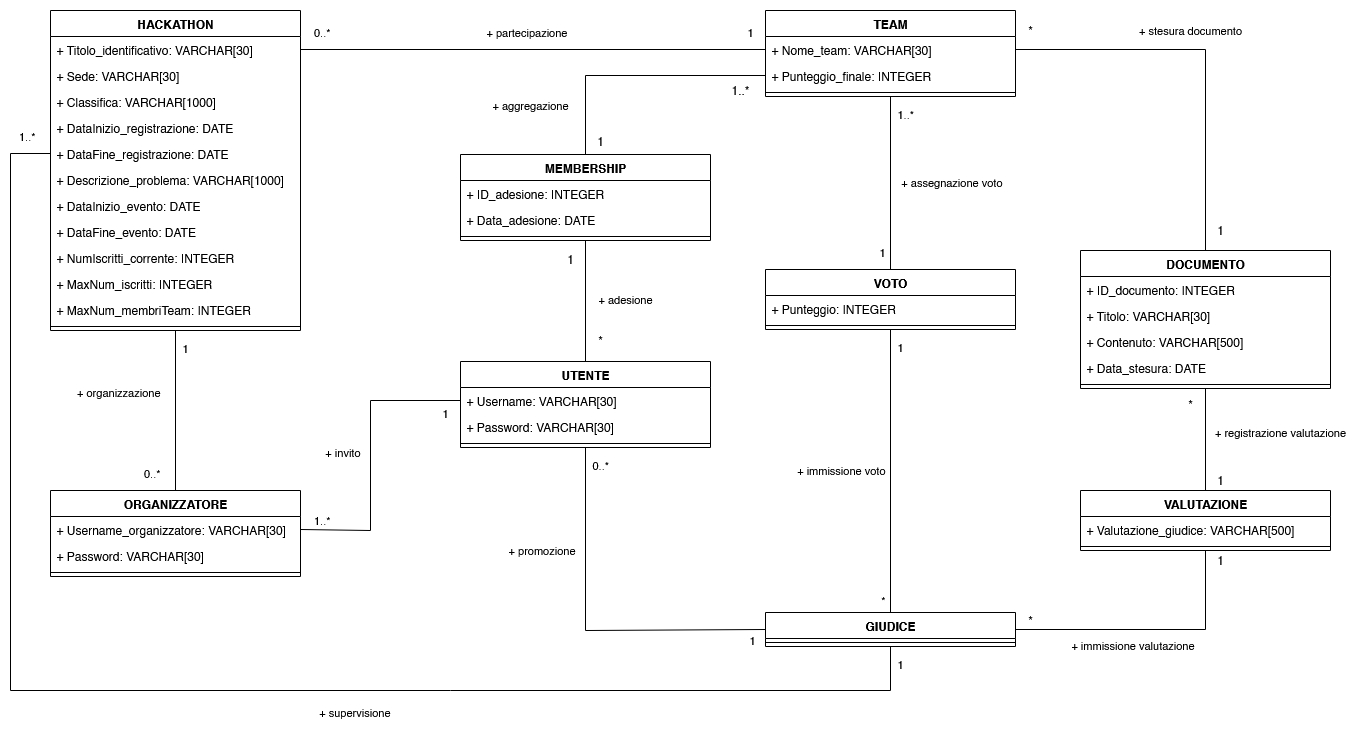
\includegraphics[width=1\textwidth]{../Immagini/Hackathon_UMLRistrutturato}
	\newpage
	\subsection{Dizionario delle Classi}
	{\footnotesize % Testo più piccolo ma leggibile
		\setlength{\arrayrulewidth}{0.5pt}  % Opzionale: regola lo spessore
		\renewcommand{\arraystretch}{1.2}  % Opzionale: aumenta lo spazio tra le righe
		\begin{longtable}{
			>{\raggedright\arraybackslash}p{4cm} % Colonna 1: allineamento a sinistra
			>{\centering\arraybackslash}p{4cm}    % Colonna 2: centrato
			>{\raggedright\arraybackslash}p{6.5cm}% Colonna 3: allineamento a sinistra
			}
			\hline
			\textbf{Classe} & \textbf{Descrizione} & \textbf{Attributi} \\
			\hline
			\endfirsthead
			\hline
			\textbf{Classe} & \textbf{Descrizione} & \textbf{Attributi} \\
			\hline
			\endhead
			\hline
			\endfoot
			\hline
			\endlastfoot
			
			\textbf{HACKATHON} &
			Evento organizzato a cui partecipano team. &
			\begin{itemize}
				\item \texttt{Titolo\_identificativo} (VARCHAR[30]): Titolo univoco che identifica un Hackathon;
				\item \texttt{Sede} (VARCHAR[30]): Sede dove si svolgerà l'Hackathon;
				\item \texttt{Classifica} (TEXT): Classifica finale con i posizionamenti dei Team, in ordine di punteggio complessivo;
				\item \texttt{DataInizio\_registrazione} (DATE);
				\item \texttt{DataFine\_registrazione} (DATE);
				\item \texttt{Descrizione\_problema} (TEXT): Descrizione del problema da risolvere offerta dai giudici;
				\item \texttt{DataInizio\_evento} (DATE);
				\item \texttt{DataFine\_evento} (DATE);
				\item \texttt{NumIscritti\_corrente} (INTEGER): Numero degli iscritti all'Hackathon aggiornato fino alla chiusura delle iscrizioni o al raggiungimento del tetto massimo;
				\item \texttt{MaxNum\_iscritti} (INTEGER): Numero massimo di iscritti per un Hackathon;
				\item \texttt{MaxNum\_membriTeam} (INTEGER): Numero massimo di membri per team iscritti ad una determinata Hackathon;
			\end{itemize} \\
			\hline
			
			\textbf{UTENTE} &
			Utente registrato nel sistema. &
			\begin{itemize}
				\item \texttt{Username} (VARCHAR[30]): Nome utente univoco;
				\item \texttt{Password} (VARCHAR[30])
			\end{itemize} \\
			\hline
			
			\textbf{ORGANIZZATORE} &
			Utente con ruolo di organizzatore. &
			\begin{itemize}
				\item \texttt{Username\_organizzatore} (VARCHAR[30]): Nome utente univoco per organizzatore;
				\item \texttt{Password} (VARCHAR[30])
			\end{itemize} \\
			\hline
			
			\textbf{GIUDICE} &
			Utente con ruolo di giudice. & \\
			\hline
			
			\textbf{TEAM} &
			Team partecipante a un hackathon. &
			\begin{itemize}
				\item \texttt{Nome\_team} (VARCHAR[30]): Nome univoco che identifica un team;
				\item \texttt{Punteggio\_finale} (INTEGER): Punteggio complessivo del team dato dalla somma di tutti i punteggi ottenuti dai giudici;
			\end{itemize} \\
			\hline
			
			\textbf{MEMBERSHIP} &
			Adesione di un utente a un team. &
			\begin{itemize}
				\item \texttt{ID\_adesione} (INTEGER): Codice identificativo per la singola adesione ad un Team;
				\item \texttt{Data\_adesione} (DATE)
			\end{itemize} \\
			\hline
			
			\textbf{VOTO} &
			Voto assegnato da un giudice a un team. &
			\begin{itemize}
				\item \texttt{Punteggio} (INTEGER)
			\end{itemize} \\
			\hline
			
			\textbf{DOCUMENTO} &
			Documento prodotto da un team. &
			\begin{itemize}
				\item \texttt{ID\_documento} (INTEGER): Codice identificativo per il singolo documento;
				\item \texttt{Titolo} (VARCHAR[30]): Titolo del documento per riassumerne il contenuto;
				\item \texttt{Contenuto} (TEXT): Testo del documento;
				\item \texttt{Data\_stesura} (DATE)
			\end{itemize} \\
			\hline
			
			\textbf{VALUTAZIONE} &
			Valutazione scritta da un giudice. &
			\begin{itemize}
				\item \texttt{Valutazione\_giudice} (TEXT): Valutazione di un giudice per un documento;
			\end{itemize} \\
			\hline
			
			\textbf{INVITO\_GIUDICE} &
			Invito a diventare Giudice da parte di un Organizzatore verso un Utente &
			\begin{itemize}
				\item \texttt{Stato\_invito} (VARCHAR[20]): Stato di un invito, diviso in tre stati: L'invito è stato inviato all'utente e attende risposta (\textit{Inviato}), l'invito è stato accettato (\textit{Accettato}), L'invito è stato rifiutato (\textit{Rifiutato});
				\item \texttt{Data\_invito} (DATE);
			\end{itemize} \\ 
		\end{longtable}
	}
	\subsection{Dizionario delle Associazioni}
	{\footnotesize
		\setlength{\arrayrulewidth}{0.5pt}
		\renewcommand{\arraystretch}{1.5}
		\begin{longtable}{
				>{\raggedright\arraybackslash}p{4cm} % Colonna 1: allineamento a sinistra
				>{\centering\arraybackslash}p{4cm}    % Colonna 2: centrato
				>{\raggedright\arraybackslash}p{6.5cm}% Colonna 3: allineamento a sinistra
			}
			\hline
			\textbf{Nome Associazione} & \textbf{Entità Associate} & \textbf{Descrizione Associazione} \\
			\hline
			\endfirsthead
			\hline
			\textbf{Nome Associazione} & \textbf{Entità Associate} & \textbf{Descrizione Associazione} \\
			\hline
			\endhead
			\hline
			\endfoot
			\hline
			\endlastfoot
			
			\textbf{Partecipazione}  & 
			HACKATHON $\leftrightarrow$ TEAM &
			\begin{itemize}
				\item Tipo: Uno-a-molti [0..1 - *]
				\item Un Hackathon può avere più Team partecipanti. Un Team deve partecipare ad un Hackathon
				\item Chiave esterna: \texttt{Titolo\_hackathon} in TEAM
				\item Vincolo: Ogni Team partecipa a un solo Hackathon
			\end{itemize} \\
			\hline
			
			\textbf{Organizzazione} & 
			ORGANIZZATORE $\leftrightarrow$ HACKATHON &
			\begin{itemize}
				\item Tipo: Uno-a-molti [0..* - 1]
				\item Un organizzatore può organizzare più Hackathon, o può non organizzarne. Un Hackathon è organizzata da un solo organizzatore
				\item Chiave esterna: \texttt{Username\_organizzatore} in ORGANIZZATORE
				\item Vincolo: Ciascun Hackathon può essere organizzata da una sola persona
			\end{itemize} \\
			\hline
			
			\textbf{Supervisione} & 
			HACKATHON $\leftrightarrow$ GIUDICE &
			\begin{itemize}
				\item Tipo: Uno-a-molti [1..* - 1]
				\item Un Hackathon può avere più Giudici assegnati
				\item Chiave esterna: \texttt{Titolo\_hackathon} in GIUDICE
				\item Vincolo: Ogni Giudice è assegnato a un solo Hackathon
			\end{itemize} \\
			\hline
			
			\textbf{Invito Giudice} & 
			ORGANIZZATORE $\leftrightarrow$ UTENTE &
			\begin{itemize}
				\item Tipo: Uno-a-molti [1..* - 1]
				\item Un organizzatore deve invitare almeno un utente a diventare giudice
				\item Vincolo: Un utente può ricevere un solo invito alla volta per essere giudice di un Hackathon
			\end{itemize} \\
			\hline
			
			\textbf{Promozione} & 
			UTENTE $\leftrightarrow$ GIUDICE &
			\begin{itemize}
				\item Tipo: Uno-a-molti [0..* - 1]
				\item Un Utente può essere promosso fino ad N volte per diventare Giudice. Un Giudice è correlato ad un solo Utente per una sola Hackathon.
				\item Vincolo: Un utente può ricevere un solo invito alla volta per essere giudice di un Hackathon
			\end{itemize} \\
			\hline
			
			\textbf{Aggregazione} & 
			TEAM $\leftrightarrow$ MEMBERSHIP &
			\begin{itemize}
				\item Tipo: Uno-a-molti [1..* - 1]
				\item Un Team può avere più adesioni (Membership)
				\item Chiave esterna: \texttt{Nome\_team} in MEMBERSHIP
				\item Vincolo: Ogni Membership è per un solo Team
			\end{itemize} \\
			\hline
			
			\textbf{Adesione} & 
			UTENTE $\leftrightarrow$ MEMBERSHIP &
			\begin{itemize}
				\item Tipo: Uno-a-molti [* - 1]
				\item Un Utente può appartenere a più Team (tramite Membership)
				\item Chiave esterna: \texttt{Username\_utente} in MEMBERSHIP
				\item Vincolo: Ogni Membership è di un solo Utente ed è rivolta ad un solo Team
			\end{itemize} \\
			\hline
			
			\textbf{Stesura Documento} & 
			TEAM $\leftrightarrow$ DOCUMENTO &
			\begin{itemize}
				\item Tipo: Uno-a-molti [* - 1]
				\item Un Team può produrre più Documenti
				\item Chiavi esterne: \texttt{Nome\_team} e \texttt{Titolo\_hackathon} in DOCUMENTO
				\item Vincolo: Ogni Documento è prodotto da un solo Team
			\end{itemize} \\
			\hline
			
			\textbf{Registrazione Valutazione} & 
			DOCUMENTO $\leftrightarrow$ VALUTAZIONE &
			\begin{itemize}
				\item Tipo: Uno-a-molti [* - 1]
				\item Un Documento può ricevere più Valutazioni
				\item Chiave esterna: \texttt{ID\_documento} in VALUTAZIONE
				\item Vincolo: Ogni Valutazione è per un solo Documento
			\end{itemize} \\
			\hline
			
			\textbf{Immissione Valutazione} & 
			GIUDICE $\leftrightarrow$ VALUTAZIONE &
			\begin{itemize}
				\item Tipo: Uno-a-molti [* - 1]
				\item Un Giudice può scrivere più Valutazioni
				\item Chiavi esterne: \texttt{ID\_giudice} e \texttt{Username\_giudice} in VALUTAZIONE
				\item Vincolo: Ogni Valutazione è scritta da un solo Giudice
			\end{itemize} \\
			\hline
			
			\textbf{Immissione Voto} & 
			GIUDICE $\leftrightarrow$ VOTO &
			\begin{itemize}
				\item Tipo: Uno-a-molti [* - 1]
				\item Un Giudice può assegnare più Voti
				\item Chiavi esterne: \texttt{ID\_giudice} e \texttt{Username\_giudice} in VOTO
				\item Vincolo: Ogni Voto è assegnato da un solo Giudice
			\end{itemize} \\
			\hline
			
			\textbf{Assegnazione Voto} & 
			TEAM $\leftrightarrow$ VOTO &
			\begin{itemize}
				\item Tipo: Uno-a-molti [1..* - 1]
				\item Un Team può ricevere più Voti
				\item Chiavi esterne: \texttt{Nome\_team} e \texttt{Titolo\_hackathon} in VOTO
				\item Vincolo: Ogni Voto è assegnato a un solo Team
			\end{itemize} \\
			\hline
		\end{longtable}
	}
	\newpage
	\subsection{Dizionario dei Vincoli}
	{\footnotesize
		\setlength{\arrayrulewidth}{0.5pt}
		\renewcommand{\arraystretch}{2.5}
		\begin{longtable}{
				>{\raggedright\arraybackslash}p{5.5cm}
				>{\raggedright\arraybackslash}p{10cm}
			}
			\hline
			\textbf{Nome Vincolo} & \textbf{Descrizione} \\
			\hline
			\endfirsthead
			\hline
			\textbf{Nome Vincolo} & \textbf{Descrizione} \\
			\hline
			\endhead
			\hline
			\endfoot
			\hline
			\endlastfoot
			
			\textbf{Password Sicura} &
			La password di un utente deve avere almeno una lettera maiuscola, una lettera minuscola, un carattere numerico, un carattere speciale e che non sia più breve di 8 caratteri \\
			\hline
			
			\textbf{Chiusura Registrazioni per Data} &
			Le registrazioni devono chiudersi 2 giorni prima dell'evento:
			\texttt{DataFine\_registrazione} = \texttt{DataInizio\_evento} - 2 giorni \\
			\hline
			
			\textbf{Chiusura Registrazioni per Limite} &
			Le registrazioni devono chiudersi quando viene raggiunto il limite massimo di iscritti all'Hackathon \\
			\hline
			
			\textbf{Coerenza Date} &
			Il periodo di registrazione all'evento non può né combaciare ne susseguire il periodo di durata dell'evento stesso.
			Le registrazioni possono avvenire solo prima dell'evento e si chiudono esattamente due giorni prima.
			Le date devono essere di per sé coerenti anche nei singoli casi: l'apertura delle registrazioni non può avvenire dopo
			la sua chiusura e viceversa, discorso analogo per l'evento.\\
			\hline
			
			\textbf{Coerenza Data di Adesione} &
			Non può esserci una data di adesione in membership che vada oltre la chiusura delle registrazioni o prima dell'apertura delle registrazioni.\\
			\hline
			
			\textbf{Range Voti} &
			I voti assegnati dai giudici devono essere interi compresi tra 0 e 10\\
			\hline
			
			\textbf{Numero Minimo Membri Team} &
			Ogni team deve avere almeno 2 membri per essere valido \\
			\hline
			
			\textbf{Numero Massimo Membri Team} &
			Un team non può superare il numero massimo di membri definito nell'Hackathon \\
			\hline
			
			\textbf{Documentazione Obbligatoria} &
			Ogni team deve aver caricato almeno un documento per essere valutato \\
			\hline
			
			\textbf{Unicità Voto Giudice} &
			Un giudice non può votare più volte lo stesso team\\
			\hline
			
			\textbf{Classifica Automatica} &
			La classifica deve essere generata automaticamente come somma dei punteggi\\
			\hline
			
			\textbf{Completezza Valutazioni} &
			Tutti i giudici devono aver votato prima della pubblicazione della classifica \\
			\hline
			
			\textbf{Blocco Team} &
			I team non possono essere modificati dopo la chiusura delle registrazioni
		\end{longtable}
	}
	\newpage
	\section{Progettazione Logica}
	\subsection{Schema Logico}
	\begin{itemize}
		\item \texttt{Hackathon(\underline{Titolo\_identificativo}, \underline{\underline{Username\_organizzatore}}, Sede, Classifica,\\
			DataInizio\_registrazione, DataFine\_registrazione, Descrizione\_problema, 
			\\DataInizio\_evento, DataFine\_evento, NumIscritti\_corrente, MaxNum\_iscritti, MaxNum\_membriTeam)}
		\begin{graybox}
			\texttt{Username\_organizzatore $\Rightarrow$ Organizzatore.Username\_organizzatore}
		\end{graybox}
		\item \texttt{Utente(\underline{Username}, Password)}
		\item \texttt{Organizzatore(\underline{Username\_organizzatore}, Password)}
		\item \texttt{Giudice(\underline{\underline{Username\_utente}}, \underline{\underline{Titolo\_hackathon}})}
		\begin{graybox}
			\texttt{Username\_utente $\Rightarrow$ Utente.Username}\\
			\texttt{Titolo\_hackathon $\Rightarrow$ Hackathon.Titolo\_identificativo}
		\end{graybox}
		\item \texttt{Team(\underline{Nome\_team}, \underline{\underline{Titolo\_hackathon}}, Punteggio\_finale)}
		\begin{graybox}
			\texttt{Titolo\_hackathon $\Rightarrow$ Hackathon.Titolo\_identificativo}
		\end{graybox}
		\item \texttt{Documento(\underline{ID\_documento}, \underline{\underline{Nome\_team}}, \underline{\underline{Titolo\_hackathon}}, Titolo,\\Contenuto, Data\_stesura)}
		\begin{graybox}
			\texttt{Nome\_team $\Rightarrow$ Team.Nome\_team}\\
			\texttt{Titolo\_hackathon $\Rightarrow$ Hackathon.Titolo\_identificativo}
		\end{graybox}
		\item \texttt{Invito\_giudice(\underline{\underline{Username\_organizzatore}}, \underline{\underline{Username\_utente}}, \underline{\underline{Titolo\_hackathon}}, Stato\_invito, Data\_invito)}
		\begin{graybox}
			\texttt{Username\_organizzatore $\Rightarrow$ Organizzatore.Username\_organizzatore} \\
			\texttt{Username\_utente $\Rightarrow$ Utente.Username}\\
			\texttt{Titolo\_hackathon $\Rightarrow$ Hackathon.Titolo\_identificativo}
		\end{graybox}
		\item \texttt{Membership(\underline{ID\_adesione}, \underline{\underline{Username\_utente}}, \underline{\underline{Nome\_team}}, \underline{\underline{Titolo\_hackathon}},\\Data\_adesione)}
		\begin{graybox}
			\texttt{Username\_utente $\Rightarrow$ Utente.Username}\\
			\texttt{Nome\_team $\Rightarrow$ Team.Nome\_team}\\
			\texttt{Titolo\_hackathon $\Rightarrow$ Hackathon.Titolo\_identificativo}
		\end{graybox}
		\item \texttt{Voto(\underline{\underline{Username\_giudice}}, \underline{\underline{Titolo\_hackathon}}, \underline{\underline{Nome\_team}}, Punteggio)}
		\begin{graybox}
			\texttt{Username\_giudice $\Rightarrow$ Utente.Username} \\
			\texttt{Titolo\_hackathon $\Rightarrow$ Hackathon.Titolo\_identificativo} \\
			\texttt{Nome\_team $\Rightarrow$ Team.Nome\_team}
		\end{graybox}
		\item \texttt{Valutazione(\underline{\underline{Username\_giudice}},\underline{\underline{Titolo\_hackathon}}, \underline{\underline{Nome\_team}}, \underline{\underline{ID\_documento}},\\Valutazione\_giudice)}
		\begin{graybox}
			\texttt{Username\_giudice $\Rightarrow$ Utente.Username} \\
			\texttt{Titolo\_hackathon $\Rightarrow$ Hackathon.Titolo\_identificativo} \\
			\texttt{Nome\_team $\Rightarrow$ Team.Nome\_team} \\
			\texttt{ID\_documento $\Rightarrow$ Documento.ID\_documento}
		\end{graybox}
	\end{itemize}
	\newpage
	\section{Progettazione Fisica}
	\subsection{Definzione Tabelle}
	In questa sezione verranno elencate le definizioni di tutte le tabelle che comporranno la nostra struttura.
	\subsubsection{Definizione di Organizzatore}
	\begin{lstlisting}[style=sqlstyle]
		CREATE TABLE ORGANIZZATORE
		(
			Username_org VARCHAR(30) PRIMARY KEY,
			Password VARCHAR(30) NOT NULL,
			-- Controllo validita password
			CONSTRAINT chk_password_complexity
			CHECK (
				-- Lunghezza minima 8 caratteri
				LENGTH(Password) >= 8 AND
				-- Almeno una lettera maiuscola
				Password ~ '[A-Z]' AND
				-- Almeno una lettera minuscola
				Password ~ '[a-z]' AND
				-- Almeno un numero
				Password ~ '[0-9]' AND
				-- Almeno un carattere speciale tra quelli consentiti
				Password ~ '[!@#$%^&*()\-_=+{};:,<.>/?]'
			)
		);
	\end{lstlisting}
	\subsubsection{Definizione di Utente}
	\begin{lstlisting}[style=sqlstyle]
		CREATE TABLE UTENTE
		(
			Username VARCHAR(30) PRIMARY KEY,
			Password VARCHAR(30) NOT NULL,
			-- Controllo validita password
			CONSTRAINT chk_password_complexity
			CHECK (
				-- Lunghezza minima 8 caratteri
				LENGTH(Password) >= 8 AND
				-- Almeno una lettera maiuscola
				Password ~ '[A-Z]' AND
				-- Almeno una lettera minuscola
				Password ~ '[a-z]' AND
				-- Almeno un numero
				Password ~ '[0-9]' AND
				-- Almeno un carattere speciale tra quelli consentiti
				Password ~ '[!@#$%^&*()\-_=+{};:,<.>/?]'
			)
		);
	\end{lstlisting}
	\newpage
	\subsubsection{Definizione di Hackathon}
	\begin{lstlisting}[style=sqlstyle]
		CREATE TABLE HACKATHON
		(
			Titolo_identificativo VARCHAR(30) PRIMARY KEY,
			Organizzatore VARCHAR(30) NOT NULL,
			Sede VARCHAR(30) NOT NULL,
			Classifica TEXT,
			DataInizio_registrazione DATE NOT NULL,
			DataFine_registrazione DATE NOT NULL,
			DataInizio_evento DATE NOT NULL,
			DataFine_evento DATE NOT NULL,
			Descrizione_problema TEXT NOT NULL,
			NumIscritti_corrente INTEGER,
			MaxNum_iscritti INTEGER NOT NULL,
			MaxNum_membriTeam INTEGER NOT NULL,
			
			FOREIGN KEY (Organizzatore) REFERENCES ORGANIZZATORE(Username_org) ON DELETE RESTRICT,
			
			-- Vincolo: la registrazione termina almeno 2 giorni prima dell'inizio dell'evento
			CHECK (DataFine_registrazione <= DataInizio_evento - INTERVAL '2 days'),
			
			-- Vincolo: l'intera registrazione deve avvenire prima dell'evento
			CHECK (DataFine_registrazione < DataInizio_evento AND DataInizio_registrazione < DataInizio_evento),
			
			-- Vincolo: le date devono risultare coerenti
			CHECK (DataInizio_registrazione < DataFine_registrazione AND DataInizio_evento < DataFine_evento)
		);
	\end{lstlisting}
	\subsubsection{Definizione di Giudice}
	\begin{lstlisting}[style=sqlstyle]
		CREATE TABLE GIUDICE
		(
			Username_utente VARCHAR(30) NOT NULL,
			Titolo_hackathon VARCHAR(30) NOT NULL,
			
			PRIMARY KEY (Username_utente, Titolo_hackathon),
			
			FOREIGN KEY (Username_utente) REFERENCES UTENTE (Username)
			ON DELETE CASCADE,
			FOREIGN KEY (Titolo_hackathon) REFERENCES HACKATHON (Titolo_identificativo)
			ON DELETE CASCADE
		);
	\end{lstlisting}
	\subsubsection{Definizione di Team}
	\begin{lstlisting}[style=sqlstyle]
		CREATE TABLE TEAM
		(
			Nome_team VARCHAR(30) UNIQUE NOT NULL,
			Punteggio_finale INTEGER,
			Titolo_hackathon VARCHAR(30) NOT NULL,
			
			PRIMARY KEY(Nome_team, Titolo_hackathon),
			
			FOREIGN KEY (Titolo_hackathon) REFERENCES HACKATHON (Titolo_identificativo)
			ON DELETE CASCADE
		);
	\end{lstlisting}
	\newpage
	\subsubsection{Definizione di Documento}
	\begin{lstlisting}[style=sqlstyle]
		CREATE TABLE DOCUMENTO
		(
			ID_documento SERIAL PRIMARY KEY,
			Nome_team VARCHAR(30) NOT NULL,
			Titolo_hackathon VARCHAR(30) NOT NULL,
			Titolo_doc VARCHAR(30) NOT NULL,
			Contenuto TEXT NOT NULL,
			Data_stesura DATE,
			
			FOREIGN KEY (Nome_team, Titolo_hackathon) REFERENCES TEAM (Nome_team, Titolo_hackathon)
			ON DELETE CASCADE
		);
	\end{lstlisting}
	\subsubsection{Definizione di Membership}
	\begin{lstlisting}[style=sqlstyle]
		CREATE TABLE MEMBERSHIP
		(
			ID_adesione SERIAL PRIMARY KEY,
			Username_utente VARCHAR(30) NOT NULL,
			Team_appartenenza VARCHAR(30) NOT NULL,
			Titolo_hackathon VARCHAR(30) NOT NULL,
			Data_adesione DATE NOT NULL,
			
			UNIQUE (Username_utente, Team_appartenenza, 
					Titolo_hackathon),
			
			FOREIGN KEY (Username_utente) 
				REFERENCES UTENTE (Username) 
				ON DELETE CASCADE,
			FOREIGN KEY (Team_appartenenza, Titolo_hackathon) 
				REFERENCES TEAM (Nome_team, Titolo_hackathon) 
				ON DELETE CASCADE
		);
	\end{lstlisting}
	\subsubsection{Definizione di Voto}
	\begin{lstlisting}[style=sqlstyle]
		CREATE TABLE VOTO
		(
			Username_giudice VARCHAR(30) NOT NULL,
			Titolo_hackathon VARCHAR(30) NOT NULL,
			Team_votato VARCHAR(30) NOT NULL,
			Punteggio INTEGER,
			
			UNIQUE (Username_giudice, Titolo_hackathon, 
				Team_votato),
				
			FOREIGN KEY (Username_giudice, Titolo_hackathon) 
				REFERENCES GIUDICE (Username_utente, Titolo_hackathon) 
				ON DELETE CASCADE,
			FOREIGN KEY (Team_votato, Titolo_hackathon) 
				REFERENCES TEAM (Nome_team, Titolo_hackathon) 
				ON DELETE CASCADE,
			
			CHECK (Punteggio >= 0 AND Punteggio <= 10)
		);
	\end{lstlisting}
	\newpage
	\subsubsection{Definizione di Valutazione}
	\begin{lstlisting}[style=sqlstyle]
		CREATE TABLE VALUTAZIONE
		(
			ID_documento INTEGER,
			Username_giudice VARCHAR(30) NOT NULL,
			Titolo_hackathon VARCHAR(30) NOT NULL,
			Team_valutato VARCHAR(30) NOT NULL,
			Valutazione_giudice TEXT,
			
			UNIQUE(ID_documento, Username_giudice, 
				Titolo_hackathon, Team_valutato),
			
			FOREIGN KEY (ID_documento) 
				REFERENCES DOCUMENTO (ID_documento) 
				ON DELETE CASCADE,
			FOREIGN KEY (Team_valutato, Titolo_hackathon) 
				REFERENCES TEAM (Nome_team, Titolo_hackathon) 
				ON DELETE CASCADE,
			FOREIGN KEY (Username_giudice, Titolo_hackathon) 
				REFERENCES GIUDICE (Username_utente, Titolo_hackathon) 
				ON DELETE CASCADE
		);
	\end{lstlisting}
	\subsubsection{Definizione di Invito Giudice}
	\begin{lstlisting}[style=sqlstyle]
		CREATE TABLE INVITO_GIUDICE
		(
			Username_organizzatore VARCHAR(30) NOT NULL,
			Username_utente VARCHAR(30) NOT NULL,
			Titolo_hackathon VARCHAR(30) NOT NULL,
			Data_invito DATE NOT NULL DEFAULT CURRENT_DATE,
			Stato_invito VARCHAR(20) NOT NULL 
				CHECK (Stato_invito IN ('Inviato', 'Accettato', 'Rifiutato')),
			
			PRIMARY KEY (Username_utente, Titolo_hackathon),
			
			FOREIGN KEY (Username_organizzatore) REFERENCES ORGANIZZATORE(Username_org) ON DELETE CASCADE,
			FOREIGN KEY (Username_utente) REFERENCES UTENTE(Username) ON DELETE CASCADE,
			FOREIGN KEY (Titolo_hackathon) REFERENCES HACKATHON(Titolo_identificativo) ON DELETE CASCADE
		);
	\end{lstlisting}
	\newpage
	\subsection{Implementazioni Vincoli}
	In questa sezione verranno riportate le implementazioni dei vincoli più complessi che non sono già stati indicati nelle definizioni delle tabelle.
	\subsubsection{Implementazione Vincolo di Creazione Giudice su Accettazione Invito}
	\begin{lstlisting}[style=sqlstyle]
		CREATE OR REPLACE FUNCTION aggiungi_giudice()
		RETURNS TRIGGER AS $$
		BEGIN
			-- Controlla se lo stato dell'invito e' diventato 'Accettato'
			IF NEW.Stato_invito = 'Accettato' THEN
				-- Inserisce il nuovo giudice, solo se non esiste gia'
				INSERT INTO GIUDICE (Username_utente, Titolo_hackathon)
				VALUES (NEW.Username_utente, NEW.Titolo_hackathon)
				ON CONFLICT DO NOTHING; -- evita errore se gia' presente
			END IF;
			RETURN NEW;
		END;
		$$ LANGUAGE plpgsql;
		
		CREATE TRIGGER trigger_aggiungi_giudice
		AFTER UPDATE ON INVITO_GIUDICE
		FOR EACH ROW
		WHEN (OLD.Stato_invito IS DISTINCT FROM NEW.Stato_invito 
			AND NEW.Stato_invito = 'Accettato')
		EXECUTE FUNCTION aggiungi_giudice();
	\end{lstlisting}
	\subsubsection{Implementazione Vincolo di Controllo sull'unicità di un Utente come Giudice}
	\begin{lstlisting}[style=sqlstyle]
		-- Funzione per verificare la sovrapposizione di date tra hackathon
		CREATE OR REPLACE FUNCTION verifica_giudice_sovrapposizione()
		RETURNS TRIGGER AS $$
		DECLARE
			nuovo_inizio DATE;
			nuovo_fine DATE;
			conteggio INTEGER;
		BEGIN
			-- Recupera le date dell'evento hackathon per cui l'utente sta diventando giudice
			SELECT h.DataInizio_evento, h.DataFine_evento
			INTO nuovo_inizio, nuovo_fine
			FROM HACKATHON h
			WHERE h.Titolo_identificativo = NEW.Titolo_hackathon;
			
			-- Verifica se l'utente e' gia' giudice per un altro hackathon con date sovrapposte
			SELECT COUNT(*)
			INTO conteggio
			FROM GIUDICE g
			JOIN HACKATHON h ON g.Titolo_hackathon = h.Titolo_identificativo
			WHERE g.Username_utente = NEW.Username_utente
			AND g.Titolo_hackathon <> NEW.Titolo_hackathon
			AND (
				-- Verifica sovrapposizione date
				(h.DataInizio_evento <= nuovo_fine AND h.DataFine_evento >= nuovo_inizio)
			);
			
			-- Se c'e' sovrapposizione, genera un errore
			IF conteggio > 0 THEN
			RAISE EXCEPTION 'L''utente % non puo'' essere giudice per questo hackathon 
				perche'' e'' gia'' giudice per un hackathon con date sovrapposte', 
				NEW.Username_utente;
			END IF;
			
			RETURN NEW;
		END;
		$$ LANGUAGE plpgsql;
		
		-- Trigger per controllare la sovrapposizione quando un utente diventa giudice
		CREATE TRIGGER trigger_verifica_giudice_sovrapposizione
		BEFORE INSERT OR UPDATE ON GIUDICE
		FOR EACH ROW
		EXECUTE FUNCTION verifica_giudice_sovrapposizione();
	\end{lstlisting}
	\subsubsection{Implementazione Vincolo di Controllo sulla validità di Adesione di un Utente ad un Team}
	\begin{lstlisting}[style=sqlstyle]
		-- Funzione per verificare se un'adesione e' valida
		CREATE OR REPLACE FUNCTION verifica_adesione_valida()
		RETURNS TRIGGER AS $$
		DECLARE
			data_fine_registrazione DATE;
			num_membri_attuali INTEGER;
			max_membri INTEGER;
			num_iscritti_corrente INTEGER;
			max_iscritti INTEGER;
		BEGIN
			-- Recupera tutti i dati necessari dall'hackathon
			SELECT h.DataFine_registrazione, h.MaxNum_membriTeam, 
			COALESCE(h.NumIscritti_corrente, 0), h.MaxNum_iscritti
			INTO data_fine_registrazione, max_membri, num_iscritti_corrente, max_iscritti
			FROM HACKATHON h
			WHERE h.Titolo_identificativo = NEW.Titolo_hackathon;
			
			-- Verifica se la data attuale e' successiva alla data di fine registrazione
			IF CURRENT_DATE > data_fine_registrazione THEN
				RAISE EXCEPTION 'Non e'' possibile aderire al team: 
					le registrazioni per l''hackathon "%" sono chiuse dal %',
				NEW.Titolo_hackathon, data_fine_registrazione;
			END IF;
			
			-- Verifica se e' stato raggiunto il numero massimo 
			-- di iscritti all'hackathon
			IF num_iscritti_corrente >= max_iscritti THEN
				RAISE EXCEPTION 'Non e'' possibile aderire al team: 
					l''hackathon "%" ha raggiunto il numero massimo di partecipanti (%)',
				NEW.Titolo_hackathon, max_iscritti;
			END IF;
			
			-- Conta il numero di membri attuali nel team
			SELECT COUNT(*)
			INTO num_membri_attuali
			FROM MEMBERSHIP m
			WHERE m.Team_appartenenza = NEW.Team_appartenenza
			AND m.Titolo_hackathon = NEW.Titolo_hackathon;
			
			-- Verifica se il team e' gia' al completo
			IF num_membri_attuali >= max_membri THEN
				RAISE EXCEPTION 'Non e'' possibile aderire al team "%": 
					il team ha gia'' raggiunto il numero massimo di membri (%)',
				NEW.Team_appartenenza, max_membri;
			END IF;
			
			-- Tutto ok, incrementa il contatore di iscritti
			UPDATE HACKATHON
			SET NumIscritti_corrente = COALESCE(NumIscritti_corrente, 0) + 1
			WHERE Titolo_identificativo = NEW.Titolo_hackathon;
			
			-- Se tutte le verifiche sono passate, permetti l'inserimento
			RETURN NEW;
		END;
		$$ LANGUAGE plpgsql;
		
		-- Trigger per controllare l'adesione al team
		CREATE TRIGGER trigger_verifica_adesione_valida
		BEFORE INSERT ON MEMBERSHIP
		FOR EACH ROW
		EXECUTE FUNCTION verifica_adesione_valida();
	\end{lstlisting}
	\subsubsection{Implementazione Vincolo di Controllo sui Team senza membri sufficienti}
	\begin{lstlisting}[style=sqlstyle]
		-- Funzione per verificare e cancellare team incompleti
		CREATE OR REPLACE FUNCTION elimina_team_incompleti()
		RETURNS void AS $$
		DECLARE
			hackathon_record RECORD;
		BEGIN
			-- Trova solo gli hackathon la cui data di fine registrazione e' OGGI
			FOR hackathon_record IN (
				SELECT h.Titolo_identificativo 
				FROM HACKATHON h 
				WHERE h.DataFine_registrazione = CURRENT_DATE
			) LOOP
				-- Elimina direttamente i team con meno di 2 membri
				DELETE FROM TEAM t
				WHERE t.Titolo_hackathon = hackathon_record.Titolo_identificativo
				AND (
					SELECT COUNT(*) 
					FROM MEMBERSHIP m 
					WHERE m.Team_appartenenza = t.Nome_team 
					AND m.Titolo_hackathon = t.Titolo_hackathon
				) < 2;
				
				RAISE NOTICE 'Eliminati tutti i team incompleti per l''hackathon "%"', 
				hackathon_record.Titolo_identificativo;
			END LOOP;
			
			RETURN;
		END;
		$$ LANGUAGE plpgsql;
	\end{lstlisting}
	\subsubsection{Implementazione Vincolo di Controllo sui Team senza Documenti caricati}
	\begin{lstlisting}[style=sqlstyle]
		-- Funzione per verificare che un team abbia caricato 
		-- almeno un documento prima di ricevere un voto
		CREATE OR REPLACE FUNCTION verifica_documento_caricato()
		RETURNS TRIGGER AS $$
		DECLARE
			documenti_count INTEGER;
		BEGIN
			-- Conta quanti documenti ha caricato il team
			SELECT COUNT(*)
			INTO documenti_count
			FROM DOCUMENTO d
			WHERE d.nome_team = NEW.team_votato
			AND d.Titolo_hackathon = NEW.Titolo_hackathon;
			
			-- Se il team non ha caricato alcun documento, 
			-- impedisci l'inserimento del voto
			IF documenti_count = 0 THEN
				RAISE EXCEPTION 'Impossibile votare il team "%": 
					non ha caricato alcun documento per l''hackathon "%"',
				NEW.team_votato, NEW.Titolo_hackathon;
			END IF;
			
			-- Se la verifica e' passata, permetti l'inserimento del voto
			RETURN NEW;
		END;
		$$ LANGUAGE plpgsql;
		
		-- Trigger per controllare che un team abbia 
		-- caricato documenti prima di ricevere un voto
		CREATE TRIGGER trigger_verifica_documento_caricato
		BEFORE INSERT ON VOTO
		FOR EACH ROW
		EXECUTE FUNCTION verifica_documento_caricato();
	\end{lstlisting}
	\subsubsection{Implementazione Funzione di Generazione della classifica finale con annessi vincoli sulla fine dell'evento e sul controllo dei giudici senza voto}
	\begin{lstlisting}[style=sqlstyle]
		-- Funzione per generare la classifica finale dell'hackathon
		CREATE OR REPLACE FUNCTION genera_classifica_hackathon(titolo_hack VARCHAR(30))
		RETURNS TEXT AS $$
		DECLARE
			classifica_text TEXT := '';
			team_record RECORD;
			posizione INTEGER := 1;
			data_fine_evento DATE;
			num_giudici INTEGER;
			num_team INTEGER;
			num_voti INTEGER;
			voti_attesi INTEGER;
		BEGIN
			-- Verifica che l'hackathon esista
			IF NOT EXISTS (SELECT 1 FROM HACKATHON WHERE Titolo_identificativo = titolo_hack) THEN
				RETURN 'Errore: Hackathon non trovato';
			END IF;
			
			-- Recupera la data di fine evento dell'hackathon
			SELECT DataFine_evento INTO data_fine_evento
			FROM HACKATHON
			WHERE Titolo_identificativo = titolo_hack;
			
			-- Verifica che l'hackathon sia terminato
			IF CURRENT_DATE < data_fine_evento THEN
				RETURN 'Errore: Non e'' possibile generare la classifica prima della fine dell''hackathon';
			END IF;
			
			-- Conta il numero di giudici per questo hackathon
			SELECT COUNT(*) INTO num_giudici
			FROM GIUDICE
			WHERE Titolo_hackathon = titolo_hack;
			
			-- Conta il numero di team per questo hackathon
			SELECT COUNT(*) INTO num_team
			FROM TEAM
			WHERE Titolo_hackathon = titolo_hack;
			
			-- Conta il numero totale di voti espressi
			SELECT COUNT(*) INTO num_voti
			FROM VOTO
			WHERE Titolo_hackathon = titolo_hack;
			
			-- Calcola il numero di voti attesi (ogni giudice deve votare ogni team)
			voti_attesi := num_giudici * num_team;
			
			-- Verifica se tutti i giudici hanno espresso il proprio voto per tutti i team
			IF num_voti < voti_attesi THEN
				RETURN 'Errore: Non e'' possibile generare la classifica. 
					Mancano ' || (voti_attesi - num_voti) || ' voti su ' 
					|| voti_attesi || ' attesi. 
					Tutti i giudici devono votare tutti i team.';
				END IF;
			
			-- Aggiorna il punteggio finale di ciascun team
			UPDATE TEAM t
			SET Punteggio_finale = (
				SELECT COALESCE(SUM(v.Punteggio), 0)
				FROM VOTO v
				WHERE v.Team_votato = t.Nome_team
				AND v.Titolo_hackathon = t.Titolo_hackathon
			)
			WHERE t.Titolo_hackathon = titolo_hack;
			
			-- Costruisce la stringa della classifica
			FOR team_record IN (
				SELECT Nome_team, Punteggio_finale
				FROM TEAM
				WHERE Titolo_hackathon = titolo_hack
				ORDER BY Punteggio_finale DESC, Nome_team ASC
			) LOOP
				classifica_text := classifica_text || 
				posizione || ' ' || 
				team_record.Nome_team || ' ' || 
				COALESCE(team_record.Punteggio_finale, 0) || E'\n';
				posizione := posizione + 1;
			END LOOP;
			
			-- Rimuovi l'ultimo carattere newline se la classifica non e' vuota
			IF LENGTH(classifica_text) > 0 THEN
				classifica_text := SUBSTRING(classifica_text, 1, LENGTH(classifica_text) - 1);
			END IF;
			
			-- Aggiorna il campo Classifica nella tabella HACKATHON
			UPDATE HACKATHON
			SET Classifica = classifica_text
			WHERE Titolo_identificativo = titolo_hack;
			
			-- Registra l'utente e la data/ora di generazione della classifica
			RAISE NOTICE 'Classifica generata da % il % UTC', 
			CURRENT_USER, TO_CHAR(
				CURRENT_TIMESTAMP AT TIME ZONE 'UTC', 'YYYY-MM-DD HH24:MI:SS'
				);
			
			RETURN classifica_text;
		END;
		$$ LANGUAGE plpgsql;
	\end{lstlisting}
	\newpage
	\subsection{Implementazione Funzioni Aggiuntive}
	\subsubsection{Implementazione Funzione per la rimozione di un Utente da un Team}
	\begin{lstlisting}[style=sqlstyle]
		-- Funzione per decrementare il contatore 
		-- quando un utente viene rimosso da un team
		CREATE OR REPLACE FUNCTION gestisci_rimozione_iscritto()
		RETURNS TRIGGER AS $$
		BEGIN
			-- Decrementa il contatore degli iscritti correnti
			UPDATE HACKATHON
			SET NumIscritti_corrente = GREATEST(COALESCE(NumIscritti_corrente, 0) - 1, 0)
			WHERE Titolo_identificativo = OLD.Titolo_hackathon;
			
			RETURN OLD;
		END;
		$$ LANGUAGE plpgsql;
		
		-- Crea trigger per decrementare il contatore quando un membro viene rimosso
		CREATE TRIGGER trigger_gestisci_rimozione_iscritto
		AFTER DELETE ON MEMBERSHIP
		FOR EACH ROW
		EXECUTE FUNCTION gestisci_rimozione_iscritto();
	\end{lstlisting}
	\subsubsection{Implementazione Funzione per la rimozione di un Team da un Hackathon}
	\begin{lstlisting}[style=sqlstyle]
		-- Funzione per gestire l'eliminazione di team completi
		CREATE OR REPLACE FUNCTION gestisci_eliminazione_team()
		RETURNS TRIGGER AS $$
		DECLARE
			num_membri INTEGER;
		BEGIN
			-- Conta quanti membri ha il team
			SELECT COUNT(*) INTO num_membri
			FROM MEMBERSHIP
			WHERE Team_appartenenza = OLD.Nome_team
			AND Titolo_hackathon = OLD.Titolo_hackathon;
			
			-- Decrementa il contatore degli iscritti per ogni membro del team
			-- Nota: facciamo l'update direttamente qui perche' il team 
			-- e tutti i suoi membri verranno eliminati insieme 
			-- a causa del vincolo ON DELETE CASCADE
			UPDATE HACKATHON
			SET NumIscritti_corrente = GREATEST(COALESCE(NumIscritti_corrente, 0) - num_membri, 0)
			WHERE Titolo_identificativo = OLD.Titolo_hackathon;
			
			RETURN OLD;
		END;
		$$ LANGUAGE plpgsql;
		
		-- Crea trigger per gestire l'eliminazione di team completi
		CREATE TRIGGER trigger_gestisci_eliminazione_team
		BEFORE DELETE ON TEAM
		FOR EACH ROW
		EXECUTE FUNCTION gestisci_eliminazione_team();
	\end{lstlisting}
	\newpage
	\subsubsection{Implementazione Funzione per l'inizializzazione del contatore degli iscritti}
	\begin{lstlisting}[style=sqlstyle]
		-- Funzione per inizializzare il contatore degli iscritti
		CREATE OR REPLACE FUNCTION inizializza_contatore_iscritti()
		RETURNS TRIGGER AS $$
		BEGIN
			-- Imposta il contatore degli iscritti a 0 se e' NULL
			NEW.NumIscritti_corrente := 0;
			RETURN NEW;
		END;
		$$ LANGUAGE plpgsql;
		
		-- Trigger per inizializzare il contatore
		CREATE TRIGGER trigger_inizializza_contatore_iscritti
		BEFORE INSERT ON HACKATHON
		FOR EACH ROW
		EXECUTE FUNCTION inizializza_contatore_iscritti();
	\end{lstlisting}
	
\end{document}
